\section{Auswertung}
\label{sec:Auswertung}

\subsection{Kallibration und Bestimmung der Effizienz}
\label{subsec:a1}
Um das Energiespektrum für unbekannte Strahler sinnvoll interpretieren zu können,
ist eine Kalibrierung der Energieskala notwendig. Dazu wird das linienreiche Spektrum eines Europium 152 Strahlers betrachtet, welches in Abbildung \ref{fig:spektrum_eu} dargestellt ist.
\begin{figure}
 \centering
 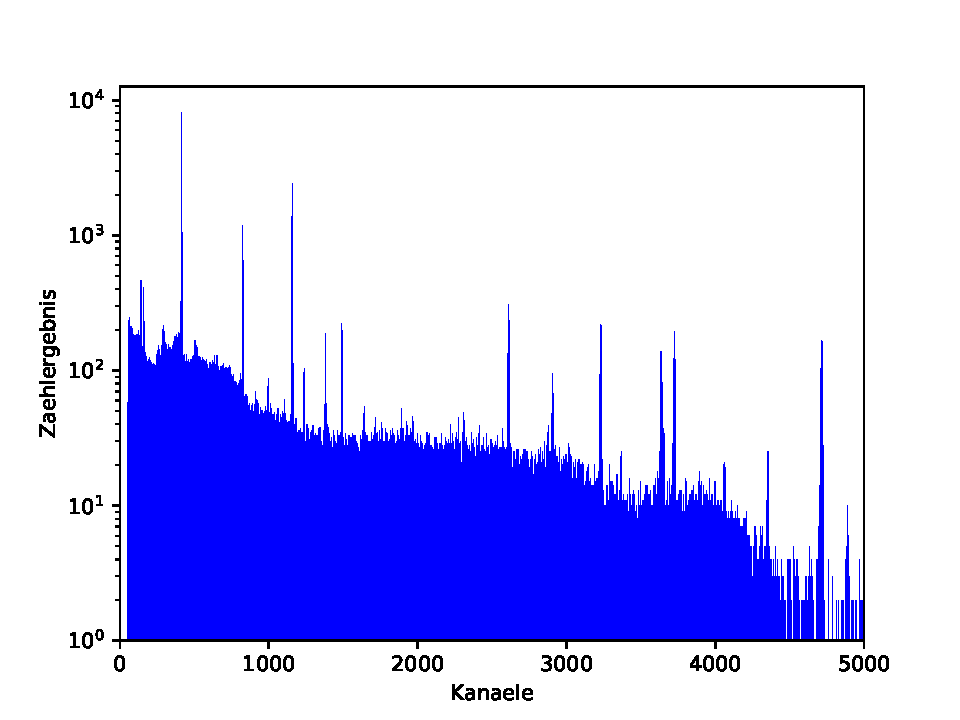
\includegraphics[width=0.8\textwidth]{python/plots/spec1.pdf}
 \caption{Rohdaten der Vermessung des Europium 152 Spektrums.}
 \label{fig:spektrum_eu}
 \end{figure} 
Die in Tabelle \ref{tab:atab1}
angegebenen Kanäle werden in Abbildung \ref{fig:Kalibrierung} gegen die Literaturwerte des Eu-Spektrums aufgetragen. 
\begin{table}
\centering
\caption{Literaturwerte und gemessene Kanäle eines Europium 152 Gammaspektrums \cite{sample}.}
\begin{tabular}{c c c}
\hline \\
Kanalnummer $k$ &Energie $E_\gamma$ in eV & Emissionswahrscheinlichkeit $W$ in \% \\
\hline \\
414.12 & 121.78 & 28.60 \\ 825.86 & 244.70 & 7.60 \\ 997.32 & 295.94 & 0.40 \\ 1158.71 & 344.30 & 26.50 \\ 1382.31 & 411.12 & 2.20 \\ 1491.59 & 443.96 & 3.10 \\ 2273.21 & 678.00 & 2.00 \\ 2310.43 & 688.67 & 0.90 \\ 2612.36 & 778.90 & 12.90 \\ 2908.55 & 867.37 & 4.20 \\ 3231.22 & 964.08 & 14.60 \\ 3368.59 & 1005.30 & 0.60 \\ 3639.40 & 1085.90 & 10.20 \\ 3726.07 & 1112.10 & 13.60 \\ 4353.21 & 1299.10 & 1.60 \\ 4716.58 & 1408.00 & 21.00 \\ 4888.94 & 1457.60 & 0.50 \\ 
\hline
\end{tabular}
\label{tab:atab1}
\end{table}
Über eine lineare Ausgleichsrechnung wird die Umrechnungsvorschrift
\begin{align*}
k(E) = s \cdot E + b \text{, mit}\\
  s = \SI{3.346+-0.001}{\per\electronvolt}\\
  b = \SI{ 5.9+-0.8}{}
\end{align*}
zwischen Kanalnummern und Energien in eV bestimmt.
Dabei wird jede Regressionsrechnung in dieser Auswertung mithilfe der Funktion \textit{curve\_ fit} aus dem Python Paket \textit{scipy.optimize} durchgeführt.
\begin{figure}
\centering
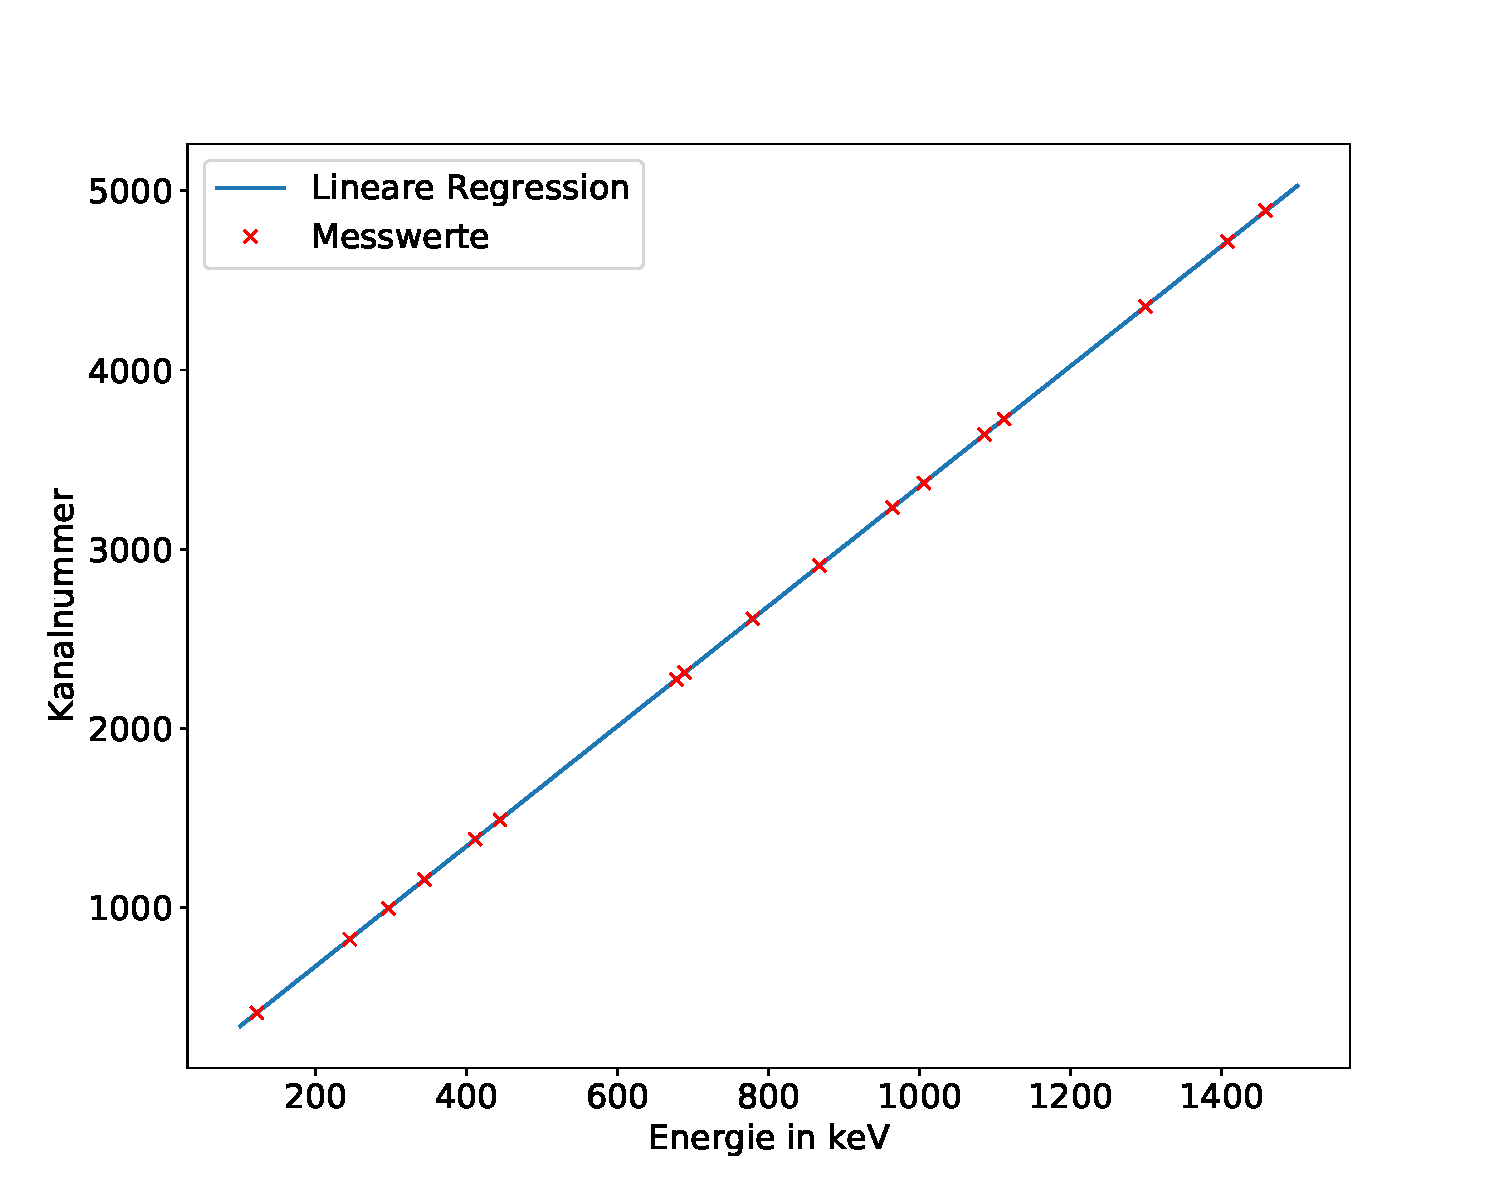
\includegraphics[width=0.8\textwidth]{python/plots/kalibrierung.pdf}
\caption{Lineare Regression der Messwerte aus Tabelle \ref{tab:atab1}}
\label{fig:Kalibrierung}
\end{figure}
Mit Gleichung \eqref{eqn:} soll die Effizienz der Spektrallinien berechnet werden.
Um die dazu nötige Aktivität des Europiums zum Zeitpunkt der Messung zu bestimmen, wird das exponentielle Zerfallsgesetz
\begin{align}
A_\text{Messung}=A_0\exp\left(\frac{\log(2)}{T_{\frac{1}{2}}}\Delta t\right)
\end{align}
verwendet.
Die Aktivität $A_0$ am 01.10.2000 betrug $\SI{130+-60}{\becquerel}$ und die Halbwertszeit von Europium beträgt $\SI{4943+-5}{\day}$ \cite{sample}.
Das angegebene Datum liefert eine zeitliche Differenz von $\Delta t=\SI{6084}{\day}$, sodass sich eine Aktivität von $A_\text{Messung}=\SI{1760+-26}{\becquerel}$ ergibt.


\begin{align*}
  A = \SI{}{\becquerel},
\end{align*}
bei einer Halbwertszeit von
\begin{align*}
  \tau = \SI{4943+-5}{\day}
\end{align*}
\subsection{Bestimmungen von Detektoreigenschaften}
\label{subsec:a2}






\subsection{Aktivitätsbestimmung von }
\label{subsec:a3}

\subsection{Untersuchung von Zerfallsketten in }
\label{subsec:a4}



%\begin{figure}
%  \centering
%  \includegraphics{plot.pdf}
%  \caption{Plot.}
%  \label{fig:plot}
%\end{figure}
